\section{Estrellas}

Las \textbf{estrellas} son de los objetos más fundamentales e importantes en el
estudio de los astros. \citetbookchapter{anIntroStellarAstro}{1} define una
estrella como \quotes{un objeto celeste en el cual existe, o alguna vez existió
(en el caso de una estrella muerta) fusión de hidrógeno sostenido en su núcleo.}
El núcleo de cada estrella activa alcanza temperaturas en el orden de decenas de
millones Kelvin, lo cual permite forjar nuevos elementos más pesados mediante el
proceso de fusión nuclear. El mecanismo principal para la generación de energía
es la fusión de hidrógeno a helio: $\ce{4 ^1H} \rightarrow \ce{^4He} + E$ .
Dentro de todas las estrellas existe un balance de fuerzas que mantiene la forma
esférica de la estrella; esto se le conoce como el \textit{equilibrio
hidrostático}, en el cual la presión interna de la estrella tiene una
contra-fuerza equivalente del peso de su mismo gas. Este balance es modelado a
escalas menores a las de las propiedades macroscópicas de la estrella
\citetbookchapter{anIntroTheoryStellarStructureEvolution}{2}, en la cual la
estrella está en un estado de \textit{equilibrio termodinámico local}. 

Una estrella es caracterizada por sus propiedades físicas, como su masa,
composición química, radio, y temperatura. A continuación se planta una base
para describir la estructura de una estrella al igual que su evolución,
empezando con la formación de una \textit{protoestrella}, la cual a lo largo del
tiempo se transforma en una estrella.

% El equilibrio termodinámico local es caracterizado por el comportamiento
% promedio de las partículas del plasma estelar. Esto se ve en las escalas del
% tiempo y el espacio de colisiones en el plasma estelar---descritos por el
% \textit{tiempo libre medio} y el \textit{camino libre medio}
% respectivamente---las cuales son mucho menor que las dimensiones de variación
% temporales y espaciales de una estrella en el caso del equilibrio local.

\subsection{Formación}

% TODO: add citations from "Formación estelar" presentation I did in MHD course
% Agrega paginas web

El \textbf{medio interestelar} (ISM por sus siglas en inglés) es la región de
espacio que existe entre el Sol y el resto de las estrellas dentro de nuestra
Galaxia. Está compuesto de todo el polvo, gas, y partículas libres como los
rayos cósmicos que atraviesan el espacio. La distribución de este material no es
uniforme a cortas escalas de distancias astronómicas, por lo cual se observan
acumulaciones de gas y polvo que se les conoce como \textbf{nubes moleculares}.
Estas nebulosas se encuentran a temperaturas extremadamente frías, hasta los
10-20 K en su estado de equilibrio. Sin embargo, la nube puede llegar a ser
perturbada de este estado, lo cual causa una distribución de masa y un campo
gravitacional no uniforme, dando forma a cúmulos densos de material.

% TODO: probably add symbols table in thesis for M_\odot (and probably others to
% be used in rest of doc)

Dado suficiente tiempo una nube molecular va colapsando bajo su propio peso,
donde la presión en la nube causa que el material se acumule en un solo punto en
el espacio. Mientras más aumente la presión el gas se calienta; este proceso
sigue hasta llegar a un equilibrio entre la presión interna del gas y la fuerza
compresiva de gravedad, en donde la nube deja de contraerse. Dependiendo de la
temperatura a la que alcanza el núcleo determina si se convierte en una estrella
capaz de mantener una reacción continua de fusión nuclear. La masa mínima para
que una nube molecular colapse a una estrella es de $0.08 \ \mathrm{M}_{\odot}$
\citetbookchapter{anIntroStellarAstro}{2}. De no cumplir con esta condición, el
cúmulo de gas y polvo no logrará mantener la cadena de reacciones termonucleares
en su núcleo, resultando en una \textit{enana café}, un objeto inerte resultado
del proceso fallido de formación estelar.

Una vez que el material de la nube se estabilice\textemdash una vez que el objeto empiece a producir energía de orden de magnitud estelar\textemdash nace una \textbf{protoestrella}. Estos objetos extensos (aproximadamente $500 \ \mathrm{R}_{\odot}$ para una protoestrella de $1 \ \mathrm{M}_{\odot}$ \citetbookchapter{astronomyPhysicalPerspective}{15}) se mantienen a una baja temperatura durante esta etapa de su vida, alrededor de 2500 K en su superficie. Sin embargo, debido a la alta densidad, la nube no es completamente transparente, por lo cual solo la superficie es capaz de liberar energía por medio de radiación infrarroja; la energía producida en su interior primero debe de viajar a la superficie por medio de convección. Conforme va evolucionando la nube se sigue comprimiendo hasta llegar a un punto en el cual puede mantener reacciones termonucleares continuas en su núcleo, llegando al punto de ser una estrella en \textbf{secuencia principal}. La \reffigure{protostarEvolutionFig} muestra la evolución de una protoestrella a una estrella secuencia principal con respecto a su temperatura y luminosidad.

\begin{figure}[!ht]
	\centering
	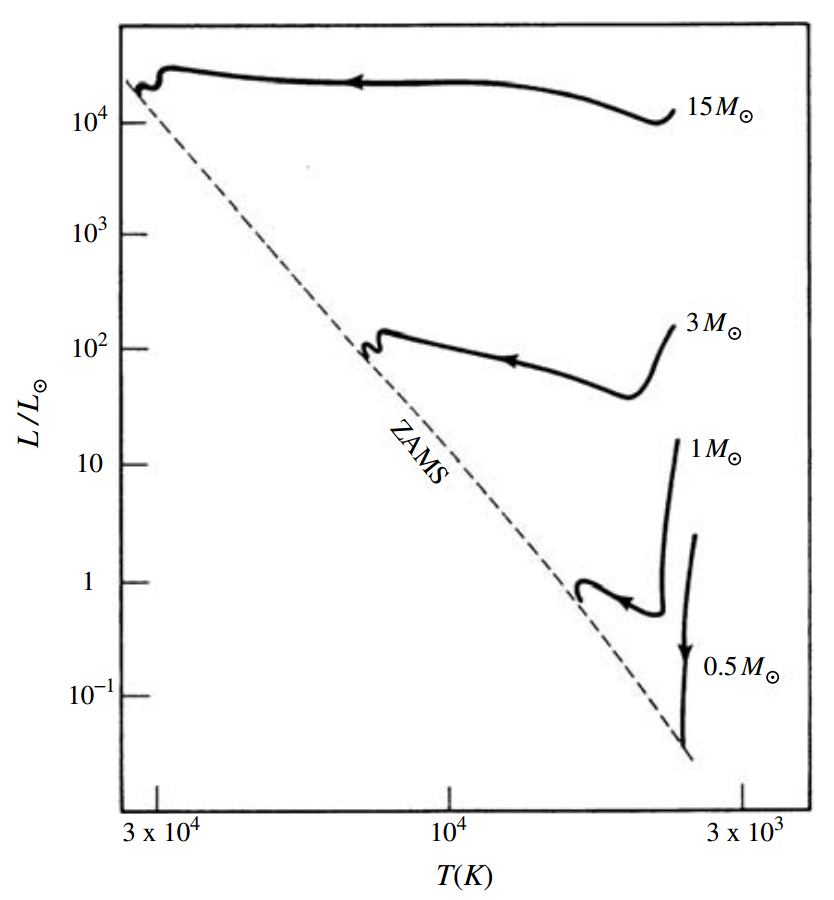
\includegraphics[scale=0.3]{Introduccion/Figures/EvolucionZAMSFormacionEstelar_Kutner.png}
	\caption{Diagrama de la evolución de una protoestrella hasta llegar a
	\textit{ZAMS} (\textit{Zero Age Main Sequence}), la edad a la que se
	convierte en una estrella de secuencia principal. Se muestran varios caminos
	evolutivos de una protoestrella en función de su masa, el cual es el
	parámetro de mayor importancia en su evolución y estado final. Figura
	obtenida de \citetbookchapter{astronomyPhysicalPerspective}{15}.}
	\label{protostarEvolutionFig}
\end{figure}

\subsection{Equilibrio Hidrostático}

\subsection{Evolución}

En el transcurso del tiempo cada estrella será sujeta a ciertos cambios en
su estructura. Esto se debe a que podemos considerar a una
estrella cómo un objeto aislado en el espacio, lo cual significa que no tendrá
algún ingreso de material significativo para reemplazar el combustible
\quotes{quemado} en las reacciones termonucleares. A lo largo del tiempo la
composición física y química de la estrella deberán cambiar para mantener el
equilibrio termodinámico.

El combustible primario de una estrella viene siendo el hidrógeno atómico, el
cual se fusiona con otros átomos (protones individuales) libres, resultando en
la producción de grandes cantidades de energía en forma de radiación y moléculas de helio como producto. El helio no es inmediatamente
util para la estrella cómo combustible, ya que requiere temperaturas más altas
de las que se encuentran durante esta fase evolutiva. Todas las estrellas conocidas pasan por esta etapa de evolución estelar;
mientras que una estrella dependa principalmente del hidrógeno para brillar se
dice que está en su etapa de \textit{secuencia principal}. 

\begin{figure}[!ht]
	\centering
	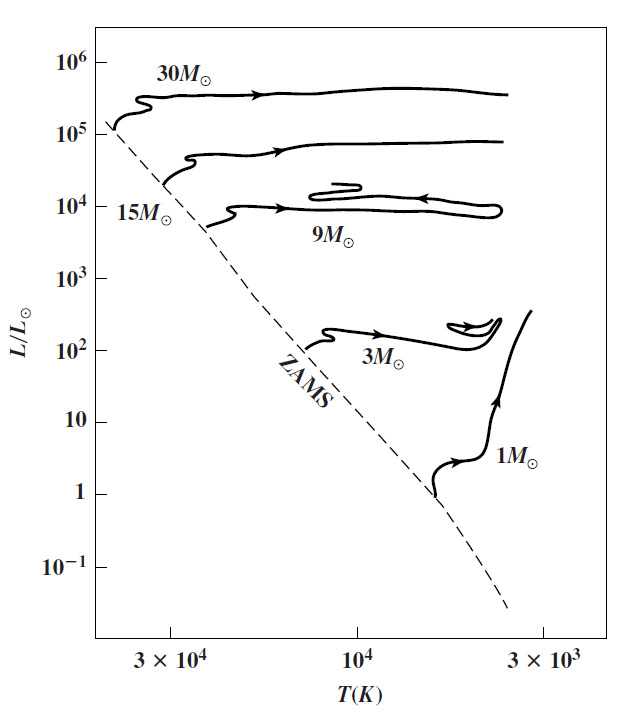
\includegraphics[scale=0.5]{Introduccion/Figures/Figura Evolucion_MS_Astronomy_Physical_Perspective.png}
	\caption{Evolución de estrellas de la secuencia principal basado en su masa
	inicial en el diagrama HR. La línea punteada representa la posición de la
	estrella en el primer momento que se integra a la secuencia principal. Al
	consumir el hidrógeno en su núcleo por las reacciones nucleares que ocurren
	en esta misma región se comienza a desatar el equilibrio delicado que
	mantiene la forma de la estrella. Esta deformación provoca una oscilación en
	su tamaño, causado por las fluctuaciones del balance entre la presión
	radiativa generada por las reacciones nucleares en el núcleo contra la
	presión gravitacional. Diagrama obtenido de \citet{astronomyPhysicalPerspective_stellarOldAgeChapter}}
	\label{evolucionMSEstrella}
\end{figure}